\begin{frame}{Strain field energy}

    \begin{columns}
        \column[T]{0.7\textwidth}

        \begin{figure}
            \centering
            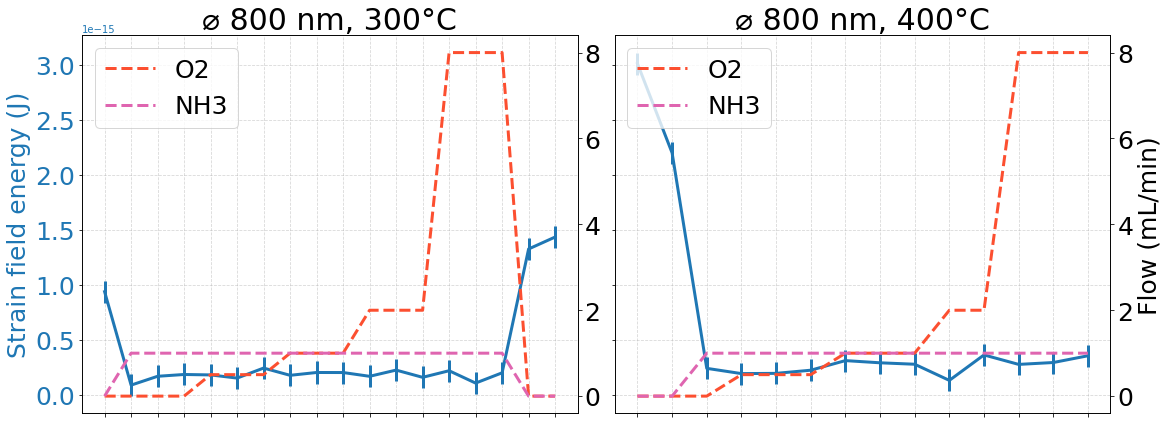
\includegraphics[width=\textwidth]{Figures/bcdi_data/D6/strain_energy_D-6.png}
            % 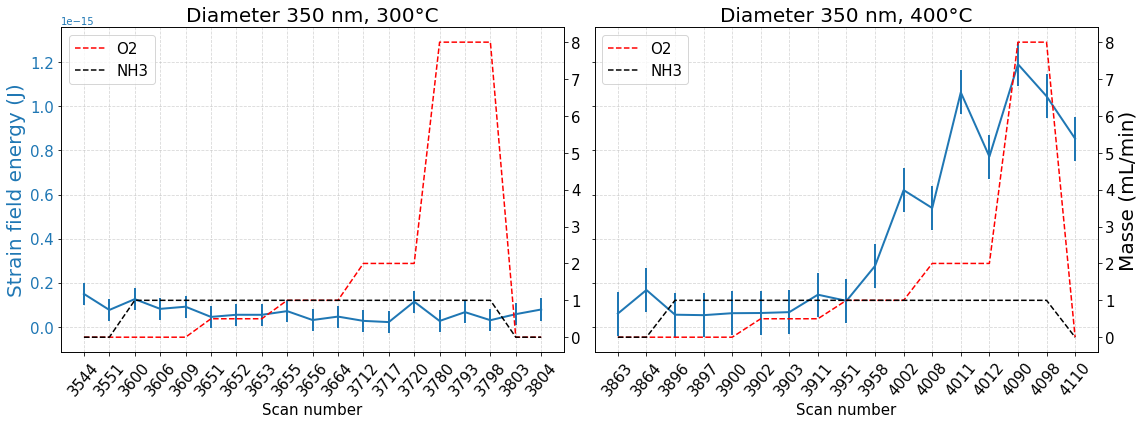
\includegraphics[width=\textwidth]{Figures/bcdi_data/B7/strain_field_B7.png}
            \onslide<2->{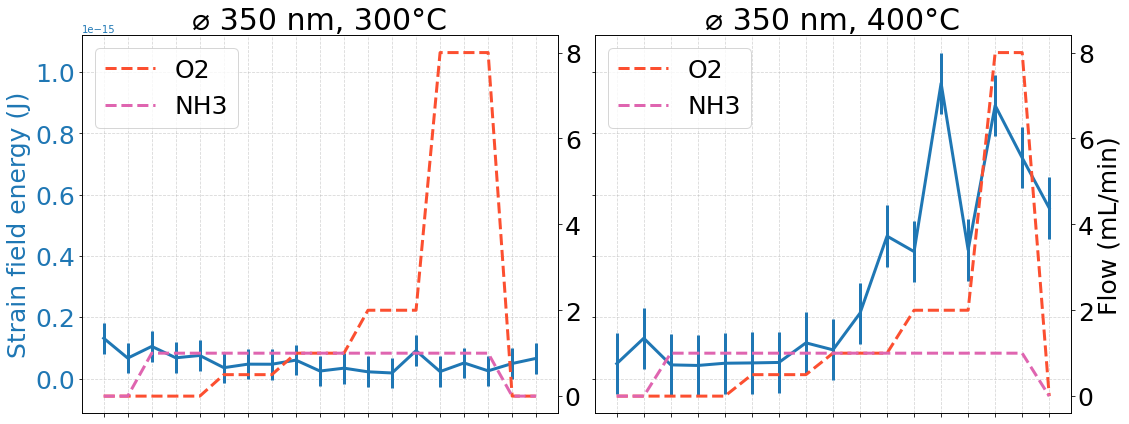
\includegraphics[width=0.51\textwidth, clip=True, trim=0 0 19.5cm 0]{Figures/bcdi_data/B7/strain_energy_B-7.png} }\hspace{-0.15cm}
            \onslide<3->{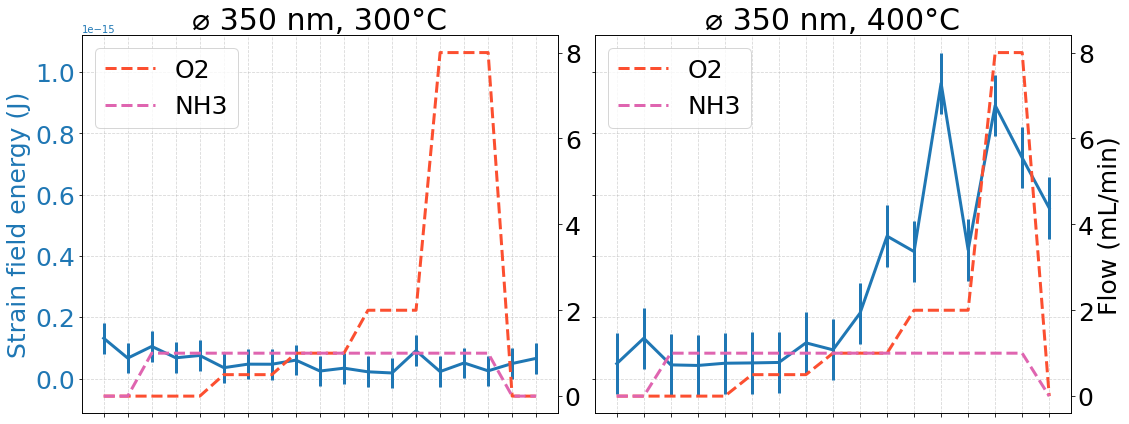
\includegraphics[width=0.48\textwidth, clip=True, trim=20.9cm 0 0 0]{Figures/bcdi_data/B7/strain_energy_B-7.png}}
            \caption{Strain field energy evolution with \ammonia and \dioxygen partial pressures.}
            \label{fig:SFE}
        \end{figure}

        \column[T]{0.3\textwidth}
        \begin{flushleft}
        \begin{equation*}
            E = \frac{A}{V} \int \Big( \frac{\partial u_{111}}{\partial x_{111}} \Big)^2dV %\frac{2G + 3I}{2}
        \end{equation*}
        \end{flushleft}

    \end{columns}
    
\end{frame}


\begin{frame}{Strain field energy}

    \begin{columns}
        \column[T]{0.7\textwidth}

        \begin{figure}
            \centering
            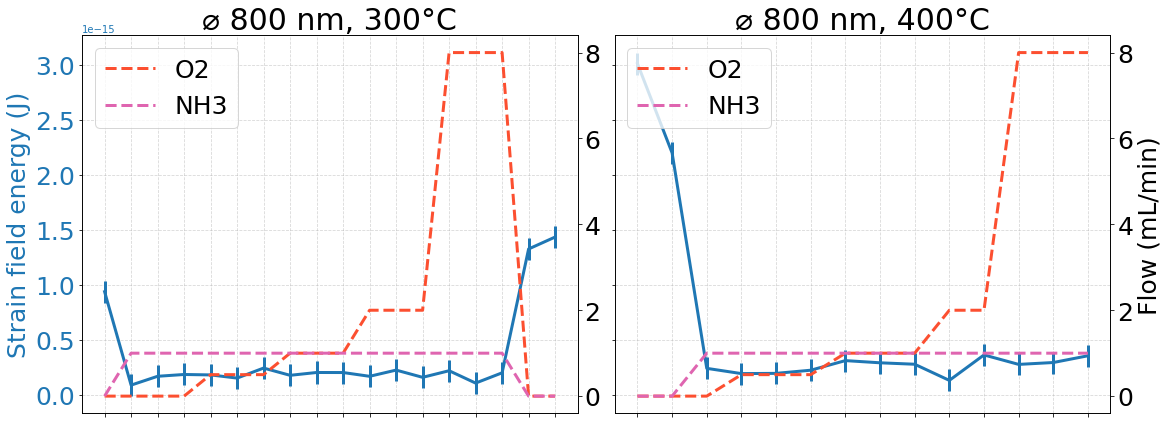
\includegraphics[width=\textwidth]{Figures/bcdi_data/D6/strain_energy_D-6.png}
            % 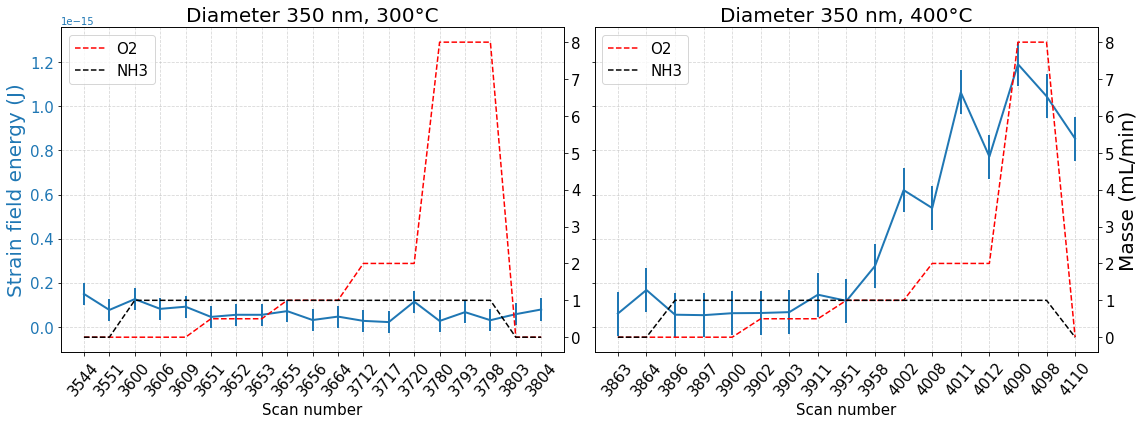
\includegraphics[width=\textwidth]{Figures/bcdi_data/B7/strain_field_B7.png}
            {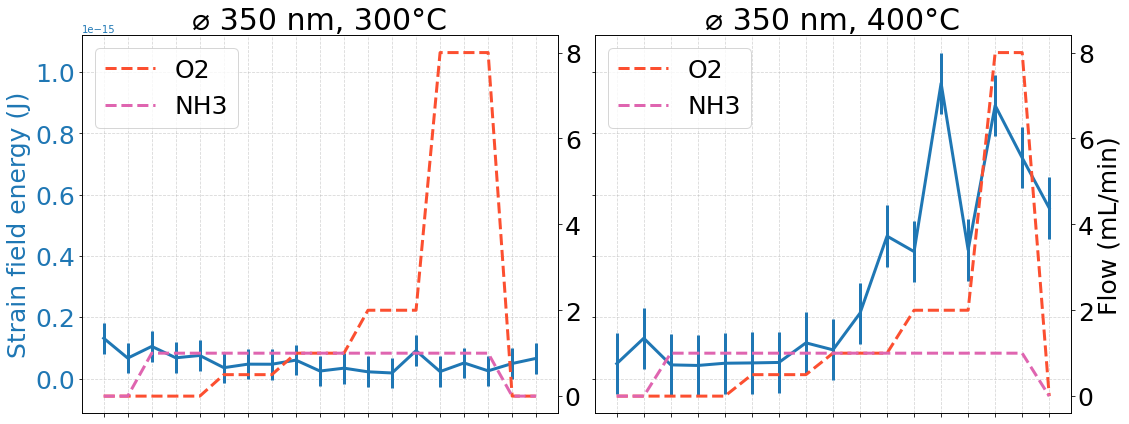
\includegraphics[width=0.51\textwidth, clip=True, trim=0 0 19.5cm 0]{Figures/bcdi_data/B7/strain_energy_B-7.png} }\hspace{-0.15cm}
            {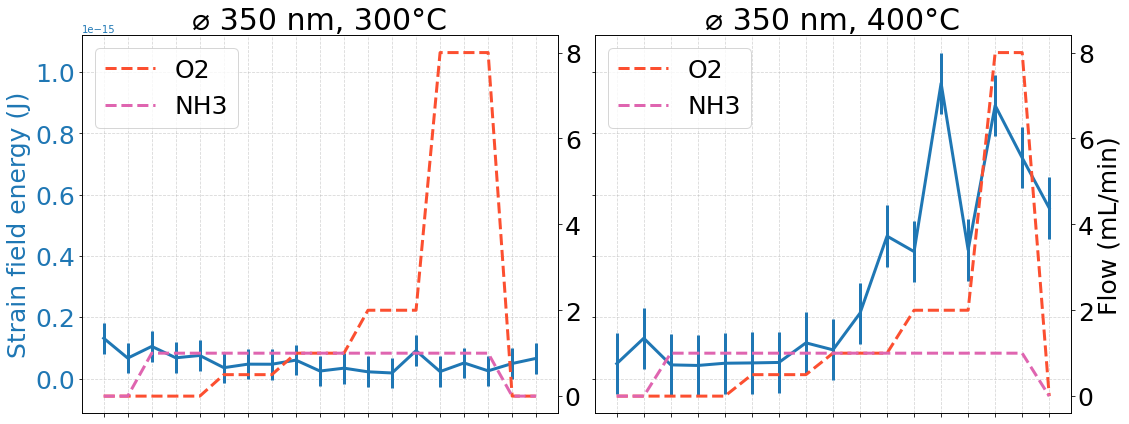
\includegraphics[width=0.48\textwidth, clip=True, trim=20.9cm 0 0 0]{Figures/bcdi_data/B7/strain_energy_B-7.png}}
            \caption{Strain field energy evolution with \ammonia and \dioxygen partial pressures.}
        \end{figure}

        \column[T]{0.3\textwidth}
        \begin{flushleft}
        \begin{equation*}
            E = \frac{A}{V} \int \Big( \frac{\partial u_{111}}{\partial x_{111}} \Big)^2dV %\frac{2G + 3I}{2}
        \end{equation*}
        \end{flushleft}
        
        \centering
        {\animategraphics[autoplay,loop, width=0.9\textwidth]{5}{Figures/bcdi_data/B7/MeshGif/3122_amp}{1}{20}}

    \end{columns}
    
\end{frame}


\begin{frame}{Strain field energy}

    \begin{columns}
        \column[T]{0.7\textwidth}

        \begin{figure}
            \centering
            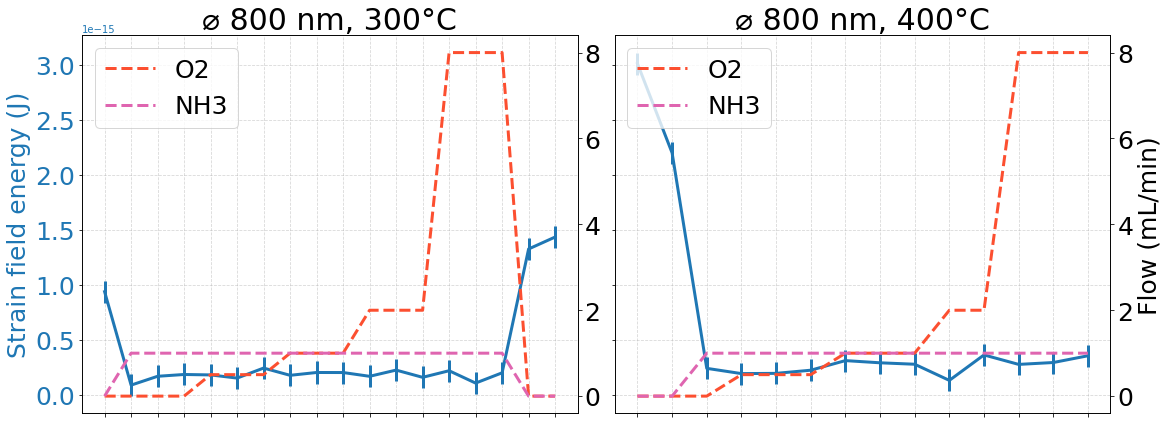
\includegraphics[width=\textwidth]{Figures/bcdi_data/D6/strain_energy_D-6.png}
            % 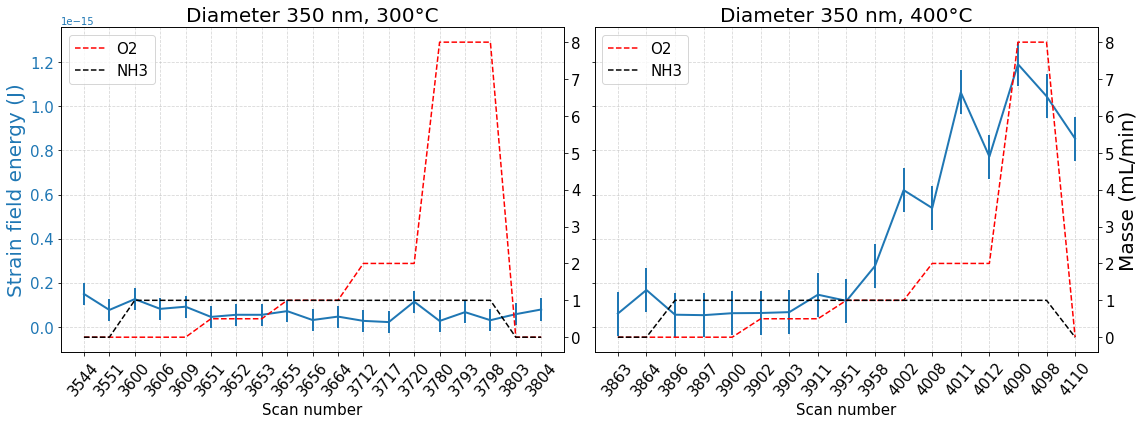
\includegraphics[width=\textwidth]{Figures/bcdi_data/B7/strain_field_B7.png}
            {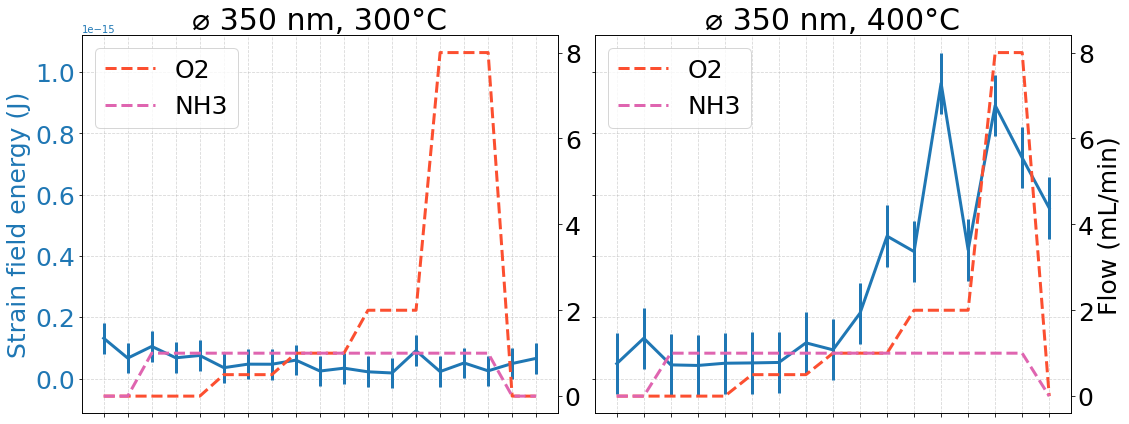
\includegraphics[width=0.51\textwidth, clip=True, trim=0 0 19.5cm 0]{Figures/bcdi_data/B7/strain_energy_B-7.png} }\hspace{-0.15cm}
            {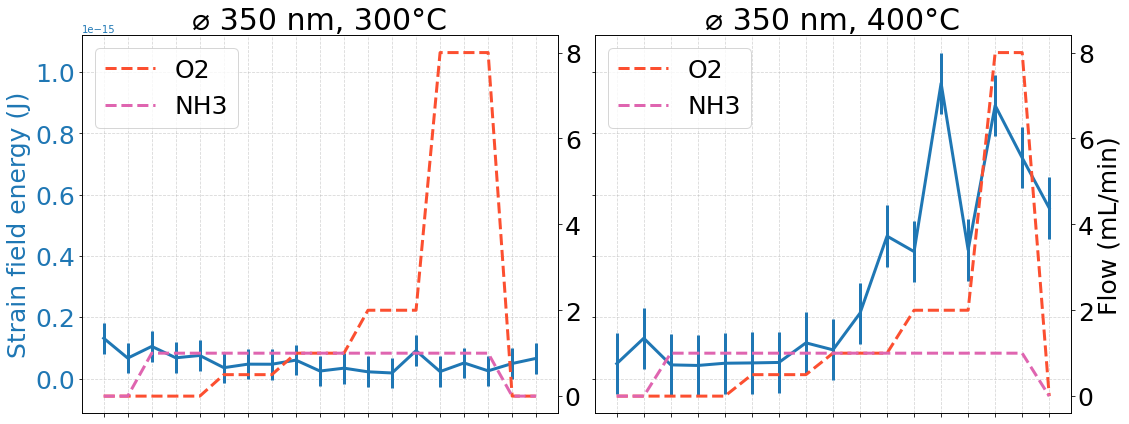
\includegraphics[width=0.48\textwidth, clip=True, trim=20.9cm 0 0 0]{Figures/bcdi_data/B7/strain_energy_B-7.png}}
            \caption{Strain field energy evolution with \ammonia and \dioxygen partial pressures.}
        \end{figure}

        \column[T]{0.3\textwidth}
        \begin{flushleft}
        \begin{equation*}
            E = \frac{A}{V} \int \Big( \frac{\partial u_{111}}{\partial x_{111}} \Big)^2dV %\frac{2G + 3I}{2}
        \end{equation*}
        \end{flushleft}
        
        \centering
        {\animategraphics[autoplay,loop, width=0.9\textwidth]{5}{Figures/bcdi_data/B7/MeshGif/3122_amp}{1}{20}}
        {\animategraphics[autoplay,loop, width=0.9\textwidth]{5}{Figures/bcdi_data/B7/MeshGif/4090_amp}{1}{20}}

    \end{columns}
    
\end{frame}